% Chapter Template

\chapter{FDTD - Three-Dimensional Scenario} % Main chapter title

\label{Chapter4} % Change X to a consecutive number; for referencing this chapter elsewhere, use \ref{ChapterX}

%----------------------------------------------------------------------------------------
%	SECTION 1
%----------------------------------------------------------------------------------------

The three-dimensional scenario has a lot of similarities with the previous versions. The methodology is again pretty much the same. It might seem a bit intimidating at first, when considering that the number of vector components to deal with has doubled. This scenario is also where optimization really matters, considering that there will be $6 \cdot N^3$ amounts of data per time step. Nonetheless, if one focuses on just the most basic implementation, taking this step by step, and splitting the effort into small parts, it will be easy to move forward.

\clearpage

\section{3D Discretization}

The easiest way to explain the 3D discretization is with Figure \ref{fig:fdtd3dDisc}.

\begin{figure}[h!]
	\centering
	\includegraphics[scale=0.6]{Figures/fdtd3dDisc}
	\decoRule
	\caption[3D Electric Discretization]{The figure shows the vectors for the electric field, with the respective magnetic vectors.}
	\label{fig:fdtd3dDisc}
\end{figure}

As seen previously, the magnetic field is staggered in every axis by half the mesh step size. The figure also gives a hint as to how the vector components are laid out in the domain. If one was to take only the electric field into the consideration, they could show where each electric vector belongs (Figure \ref{fig:fdtd3dFull}). 

\begin{figure}[h!]
	\centering
	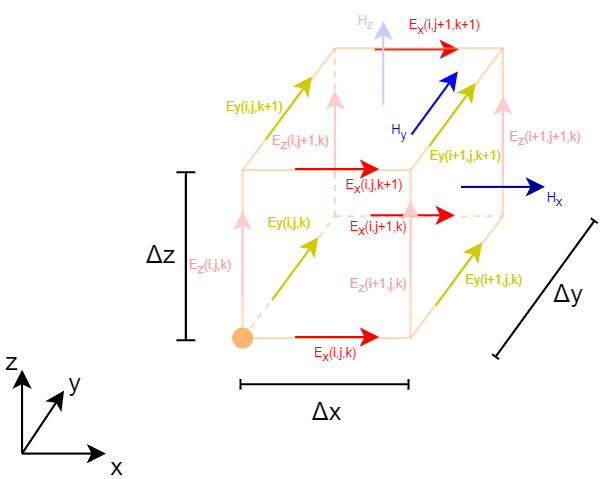
\includegraphics[scale=0.6]{Figures/fdtd3dFull}
	\decoRule
	\caption[3D Electric Discretization]{The figure shows the vectors for the electric field, with the respective magnetic vectors.}
	\label{fig:fdtd3dFull}
\end{figure}

Despite the fact that the image above is fairly cluttered with information, only bits of it are needed at a time. A keen eye will notice in the next section that the electromagnetic curls for the three-dimensional scenario can be derived in the same way that was used for the two-dimensional scenario.

%-----------------------------------
%	SUBSECTION 1
%-----------------------------------
\subsection{3D Electromagnetic Curls}

In the previous chapter, the vector curl for $H_z$ was derived, resulting in the update equation for the magnetic field. Luckily the curl is exactly the same in the three-dimensional scenario, however the formula needs to be revised to account for the added dimension, starting by changing the indexing scheme to the following:

\begin{equation}
	\label{eqn:indexing3DElectric}
	E_{i,j,k} = E(i \cdot \Delta x , j \cdot \Delta y, k \cdot \Delta z)
\end{equation}

From there, the same process as before can be repeated.
\begin{multline}
	\label{eqn:3dHzCurl1}
	\oint \vec{E} \cdot d\vec{s} = - \frac{d}{dt} \iint \mu \cdot \vec{H} \cdot d\vec{A} \\
	\Rightarrow E_x(i,j,k) \cdot \Delta x - E_x(i,j+1,k) \cdot \Delta x + E_y(i+1,j,k) \cdot \Delta y - E_y(i,j,k) \cdot \Delta y \\ = -\frac{d}{dt}(\mu \cdot H_z(i,j,k) \cdot \Delta x \cdot \Delta y)
\end{multline}

\begin{equation}
	\label{eqn:3dHzCurl2}
	\frac{d}{dt} H_z(i,j,k) = -\frac{1}{\mu} \cdot (\frac{E_x(i,j,k) - E_x(i,j+1,k)}{\Delta y} + \frac{E_y(i+1,j,k)- E_y(i,j,k)}{\Delta x})
\end{equation}

Using a uniform mesh size again, $\Delta x = \Delta y =  \Delta z = \Delta s$, equation \ref{eqn:3dHzCurl2} can be simplified to:

\begin{equation}
	\label{eqn:3dHzCurl3}
	\frac{d}{dt} H_z(i,j,k) = -\frac{1}{\mu \cdot \Delta s} \cdot ((E_x(i,j,k) - E_x(i,j+1,k) + E_y(i+1,j,k)- E_y(i,j,k))
\end{equation}

For the left hand side:

\begin{equation}
	\label{eqn:3dHzCurl4}
	\frac{d}{dt} H_z(i,j,k) = \frac{H_z^{new}(i,j,k) - H_z^{prev}(i,j,k)}{\Delta t}
\end{equation}

And finally:
\begin{multline}
	\label{eqn:3dHzCurlFinal}
	H_z^{new}(i,j,k) =  H_z^{prev}(i,j,k) + \frac{\Delta t}{\mu \cdot \Delta s} \cdot \\ (E_x(i,j+1,k) - E_x(i,j,k) - E_y(i+1,j,k) + E_y(i,j,k))
\end{multline}

Using the same method, one can obtain the update equation for the $H_y$ curl in Figure \ref{fig:fdtd3dHyCurl}

\begin{figure}[h!]
	\centering
	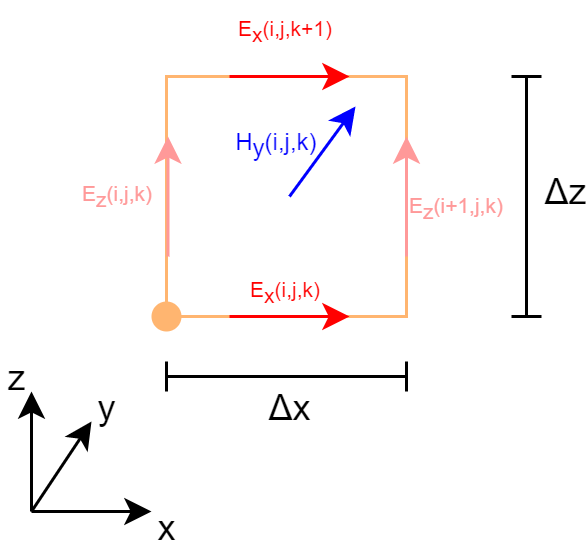
\includegraphics[scale=0.5]{Figures/fdtd3dHyCurl}
	\decoRule
	\caption[3D $H_y$ vector curl]{The curl around the magnetic field vector $H_y$.}
	\label{fig:fdtd3dHyCurl}
\end{figure}

It can be noted that the magnetic vector $H_y(i,j,k)$ is affected by the electric vectors $E_x(i,j,k), E_x(i,j,k+1), E_z(i,j,k)$, and $E_z(i+1,j,k)$. The resulting update equation will then be:
\begin{multline}
	\label{eqn:3dHyCurlFinal}
	H_y^{new}(i,j,k) =  H_y^{prev}(i,j,k) + \frac{\Delta t}{\mu \cdot \Delta s} \cdot \\ (E_z(i+1,j,k) - E_z(i,j,k) - E_x(i,j,k+1) + E_x(i,j,k))
\end{multline}

Before continuing with the magnetic field, let's quickly take a look at the electric vector $E_z$ curl (Figure \ref{fig:fdtd3dEzCurl}). The reasons for this will become apparent shortly.

\begin{figure}[h!]
	\centering
	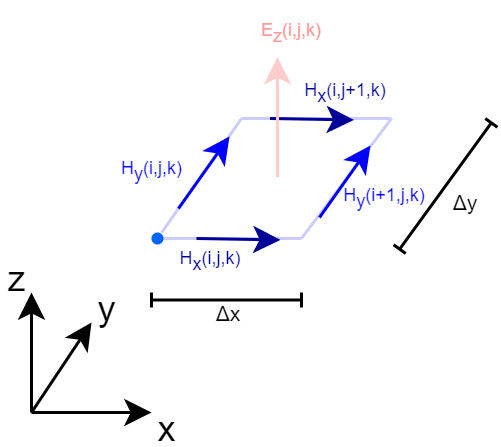
\includegraphics[scale=0.5]{Figures/fdtd3dEzCurl}
	\decoRule
	\caption[3D $E_z$ vector curl]{The curl around the electric field vector $E_z$.}
	\label{fig:fdtd3dEzCurl}
\end{figure}

Once more, as the case was in the previous chapter, the methodology here is the same. One must however now account for not only the added dimension, but also the fact that previously one of the magnetic vectors was zero.
Starting off from the initial Maxwell equation:

\begin{equation}
	\label{eqn:magneticIntegral}
	\oint \vec{H} \cdot d\vec{s} = \frac{d}{dt} \iint \epsilon \cdot \vec{E} \cdot d\vec{A}
\end{equation}
\begin{multline}
	\label{eqn:3dEzCurl1}
	\Rightarrow H_x(i,j-1,k) \cdot \Delta x + H_y(i,j,k) \cdot \Delta y - H_x(i,j,k) \cdot \Delta x - H_y(i-1,j,k) \cdot \Delta y =\\ \epsilon \cdot \frac{d}{dt} E_z(i,j,k) \cdot \Delta x \cdot \Delta z
\end{multline}

Again taking into account the uniform mesh:
\begin{equation}
	\label{eqn:3dEzCurl2}
	\frac{d E_z(i,j,k)}{dt} = \frac{1}{\epsilon \Delta s} (H_x(i,j-1,k) + H_y(i,j,k) - H_x(i,j,k) - H_y(i-1,j,k))
\end{equation}

On the left hand side:
\begin{equation}
	\label{eqn:3dEzCurl3}
	\frac{d E_z(i,j,k)}{dt} = \frac{E_z^{new}(i,j,k) - E_z^{prev}(i,j,k)}{\Delta t}
\end{equation}

Finally, by combining equation \ref{eqn:3dEzCurl2} and \ref{eqn:3dEzCurl3}:
\begin{multline}
	\label{eqn:3dEzCurlFinal}
	E_z^{new}(i,j,k) =  E_z^{prev}(i,j,k) + \frac{\Delta t}{\epsilon \cdot \Delta s} \cdot \\ (H_x(i,j-1,k) - H_x(i,j,k) - H_y(i-1,j,k) + H_y(i,j,k))
\end{multline}

One could proceed to manually do the curls for the remaining field vectors, however with a keen eye a pattern can be noticed in the equations above, shown in formula \ref{eqn:3dCurlPattern}.
\begin{multline}
	\label{eqn:3dCurlPattern}
	V_{a_1}^{new}(i,j,k) =  V_{a_1}^{prev}(i,j,k) + \frac{\Delta t}{\alpha \cdot \Delta s} \cdot \\ (T_{a_2}(C_1) - T_{a_2}(i,j,k) - T_{a_3}(C_2) + T_{a_3}(i,j,k))
\end{multline}

where:

\begin{itemize}
	\item \textbf{V} is the vector field type, which can be either \textbf{E} or \textbf{H}
	\item \textbf{T} is the opposite of \textbf{V}, meaning if $V = E$, then $T = H$
	\item $\boldsymbol{a_1,a_2,a_3}$ symbolize the axes, which need to follow a specific order: $x,y,z,x,y,z,x...$ . As an example, if $a_1 = y$, then $a_2 = z$ and $a_3 = x$
	\item $\boldsymbol{\alpha}$ is either $\epsilon$ when calculating for an electric field vector, or $\mu$ for a magnetic one.
	\item $\boldsymbol{C_1, C_2}$ are the indexes of the vectors that are shifted by one in the direction of an axis, which depend on two things: which axis the vector is parallel to, and whether the calculation is being done for an electric field or a magnetic one.
\end{itemize}

The last point deserves a deeper explanation in order to be elaborated properly. $C_1$ and $C_2$ are indexes of type (i,j,k), where one of the indexes is $\pm1$. If the equation for the electric curl is being calculated, the sign will be $+$. Otherwise it will be $-$. The updated index, meaning the one that will have the $\pm1$, will be the index that belongs to neither the vector that the equation is for, nor the vector to which the curl belongs to.

The $H_x$ vector curl, shown in Figure \ref{fig:fdtd3dHxCurl}, can be used to test this pattern.

\begin{figure}[h!]
	\centering
	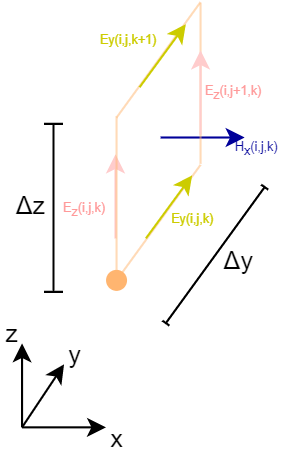
\includegraphics[scale=0.6]{Figures/fdtd3dHxCurl}
	\decoRule
	\caption[3D $H_x$ vector curl]{The curl around the magnetic field vector $H_x$.}
	\label{fig:fdtd3dHxCurl}
\end{figure}

From the image, the following can be deduced:

\begin{enumerate}
	\item $V = H$
	\item $T = E$
	\item $a_1 = x$, meaning $a_2 = y$ and $a_3 = z$
	\item $\alpha = \mu$
	\item $C_1$ in this case are the indexes for $E_y$. Since this is the curl for $H_x$, that means the $z$ index is being increased by one, meaning that $C_1$ needs to be replaced with $i,j,k+1$
	\item Similarly, $C_2$ would be replaced by $i,j+1,k$\\
\end{enumerate}

The resulting equation would then be:
\begin{multline}
	\label{eqn:3dHxPatternFinal}
	H_x^{new}(i,j,k) =  H_x^{prev}(i,j,k) + \frac{\Delta t}{\mu \cdot \Delta s} \cdot \\ (E_y(i,j,k+1) - E_y(i,j,k) - E_z(i,j+1,k) + E_z(i,j,k))
\end{multline}

To confirm that the equation is the same, after doing the curls the result would be:
\begin{multline}
	\label{eqn:3dHxCurl1}
	H_x^{new}(i,j,k) =  H_x^{prev}(i,j,k) - \frac{\Delta t}{\mu \cdot \Delta s} \cdot \\ (E_y(i,j,k) + E_z(i,j,k) - E_y(i,j,k+1) - E_z(i,j,k))
\end{multline}

On the right hand side, the $-$ sign the second half of the equation can be flipped by multiplying the curl in the brackets by $-1$:
\begin{multline}
	\label{eqn:3dHxCurl2}
	H_x^{new}(i,j,k) =  H_x^{prev}(i,j,k) + \frac{\Delta t}{\mu \cdot \Delta s} \cdot \\ -1 \cdot (E_y(i,j,k) + E_z(i,j,k) - E_y(i,j,k+1) - E_z(i,j,k))
\end{multline}

Now, by working only with the curl part:
\begin{multline}
	-1 \cdot (E_y(i,j,k) + E_z(i,j,k) - E_y(i,j,k+1) - E_z(i,j,k)) \\
	\Leftrightarrow (- E_y(i,j,k) - E_z(i,j,k) + E_y(i,j,k+1) + E_z(i,j,k)) \\
	\Leftrightarrow (E_y(i,j,k+1) - E_y(i,j,k) - E_z(i,j+1,k) + E_z(i,j,k))
\end{multline}

Therefore, the final equation is:
\begin{multline}
	\label{eqn:3dHxCurlFinal}
	H_x^{new}(i,j,k) =  H_x^{prev}(i,j,k) + \frac{\Delta t}{\mu \cdot \Delta s} \cdot \\ (E_y(i,j,k+1) - E_y(i,j,k) - E_z(i,j+1,k) + E_z(i,j,k))
\end{multline}

which is equal to equation \ref{eqn:3dHxPatternFinal}.

By using either method, one can derive the update equations for the vectors that have not been determined yet: $E_x$ (\ref{eqn:3dExCurlFinal}) and $E_y$ (\ref{eqn:3dEyCurlFinal}).
\begin{multline}
	\label{eqn:3dExCurlFinal}
	E_x^{new}(i,j,k) =  E_x^{prev}(i,j,k) + \frac{\Delta t}{\mu \cdot \Delta s} \cdot \\ (H_y(i,j,k-1) - H_y(i,j,k) - H_z(i,j-1,k) + H_z(i,j,k))
\end{multline}
\begin{multline}
	\label{eqn:3dEyCurlFinal}
	E_y^{new}(i,j,k) =  E_y^{prev}(i,j,k) + \frac{\Delta t}{\mu \cdot \Delta s} \cdot \\ (H_z(i-1,j,k) - H_z(i,j,k) - H_x(i,j,k-1) + H_x(i,j,k))
\end{multline}

Next is the code implementation.

%----------------------------------------------------------------------------------------
%	SECTION 2
%----------------------------------------------------------------------------------------

\section{C++ Implementation}

Starting from the two-dimensional implementation, few changes need to be made in order to adapt the program for three dimensions. If the previous code is used as a basis, then all the header files that are neeeded as well as the basic code structure are already there. One can immediately take a look at which environment variables will need changing.

\begin{minted}[breaklines,frame=single,fontsize=\footnotesize]{c++}
int N = 50;
int iterNum = 200;
\end{minted}

It is highly recommended to drastically reduce the size of the domain as well as the number of iterations. The reason is that not only have  the amount of update loops increased from $N^2$ to $N^3$, but now there are also six three-dimensional C++ vectors instead of three two-dimensional ones. It is recommended to start from a small number and go up for there. The hardware that is available to the author of this project can handle around this much, so these values will stay as they are for now. It is a good thing to note that the resulting files can be too big for Paraview to handle, so that is another limitation there.

Now that there are three dimensions, the \textit{deltaT} equation will also need to be updated:

\begin{minted}[breaklines,frame=single,fontsize=\footnotesize]{c++}
double deltaT = (deltaZ * sqrt(permitivity*permeability)  * (1/sqrt(3)));
\end{minted}

Furthermore, six three-dimensional C++ vectors are needed for the electric and magnetic fields, all initialized with N zeros in each entry:

\begin{minted}[breaklines,frame=single,fontsize=\footnotesize]{c++}
vector<vector<vector<double>>> Ex(N, vector<vector<double>>(N, vector<double>(N, 0)));
vector<vector<vector<double>>> Ey(N, vector<vector<double>>(N, vector<double>(N, 0)));
vector<vector<vector<double>>> Ez(N, vector<vector<double>>(N, vector<double>(N, 0)));
vector<vector<vector<double>>> Hx(N, vector<vector<double>>(N, vector<double>(N, 0)));
vector<vector<vector<double>>> Hy(N, vector<vector<double>>(N, vector<double>(N, 0)));
vector<vector<vector<double>>> Hz(N, vector<vector<double>>(N, vector<double>(N, 0)));
\end{minted}

Next the functions that create CSV files for the data need to be modified. Now that there is an equal number of vectors for both the electric and the magnetic wave, only one function is needed to handle both fields:

\begin{minted}[breaklines,frame=single,fontsize=\footnotesize]{c++}
void writeDataToCsvFile(string filename, const vector<vector<vector<double>>> &Vx, const vector<vector<vector<double>>> &Vy, const vector<vector<vector<double>>> &Vz){
	
	//	x,y,z,Vx,Vy,Vz
	//	0,0,Vx[x,y,z],Vy[x,y,z],Vz[x,y,z]
	
	ofstream csvFile(filename);
	csvFile << "x,y,z,Vx,Vy,Vz\n";
	
	for (unsigned  x = 0; x < Vx[0][0].size(); x++) {
		for (unsigned  y = 0; y < Vy[x][0].size(); y++) {
			for (unsigned  z = 0; z < Vz[x][y].size(); z++) {
				csvFile << x << "," << y << "," << z << "," << Vx[x][y][z] << "," << Vy[x][y][z] << "," << Vz[x][y][z] << "\n";
			}
		}
	}
	
	csvFile.close();
}
\end{minted}

For the main loop, one can choose to apply the Gaussian Pulse excitation to either an electric field vector or the magnetic one. Both work, however when using the magnetic field for the excitation, it may be necessary to lower the magnitude if using vacuum as a medium. Depending on the material used in the domain, this may be unnecessary. Once more, applying this excitation in the middle of the vector results in a nice symmetrical wave propagation.

\begin{minted}[breaklines,frame=single,fontsize=\footnotesize]{c++}
Ex[24][24][24] = exp(-(beta * pow((t - gamma), 2)));
\end{minted}

Only one of the field vectors is needed to apply the excitation, however which one is chosen will affect the order of the update loops. If using an electric vector for the excitation, the loop order is as follows:

\begin{minted}[breaklines,frame=single,fontsize=\footnotesize]{c++}
// loop for values
for (int i = 0; i < N-1; i++) {
	for (int j = 0; j < N-2; j++) {
		for (int k = 0; k < N-2; k++) {
			Hx[i][j][k] = Hx[i][j][k] + (deltaT / permeability / deltaZ) * (Ey[i][j][k+1] - Ey[i][j][k] - Ez[i][j+1][k] + Ez[i][j][k]);
		}
	}
}

for (int i = 0; i < N-2; i++) {
	for (int j = 0; j < N-1; j++) {
		for (int k = 0; k < N-2; k++) {
			Hy[i][j][k] = Hy[i][j][k] + (deltaT / permeability / deltaZ) * (Ez[i+1][j][k] - Ez[i][j][k] - Ex[i][j][k+1] + Ex[i][j][k]);
		}
	}
}

for (int i = 0; i < N-2; i++) {
	for (int j = 0; j < N-2; j++) {
		for (int k = 0; k < N-1; k++) {
			Hz[i][j][k] = Hz[i][j][k] + (deltaT / permeability / deltaZ) * (Ex[i][j+1][k] - Ex[i][j][k] - Ey[i+1][j][k] + Ey[i][j][k]);
		}
	}
}

writeDataToCsvFile((filePath + "H/H.csv." + to_string(i)), Hx, Hy, Hz);

for (int i = 0; i < N-1; i++) {
	for (int j = 1; j < N-1; j++) {
		for (int k = 1; k < N-1; k++) {
			Ex[i][j][k] = Ex[i][j][k] + (deltaT / permitivity / deltaZ) * (Hy[i][j][k-1] - Hy[i][j][k] - Hz[i][j-1][k] + Hz[i][j][k] );
		}
	}
}

for (int i = 1; i < N-1; i++) {
	for (int j = 0; j < N-1; j++) {
		for (int k = 1; k < N-1; k++) {
			Ey[i][j][k] = Ey[i][j][k] + (deltaT / permitivity / deltaZ) * (Hz[i-1][j][k] - Hz[i][j][k] - Hx[i][j][k-1] + Hx[i][j][k]);
		}
	}
}

for (int i = 1; i < N-1; i++) {
	for (int j = 1; j < N-1; j++) {
		for (int k = 0; k < N-1; k++) {
			Ez[i][j][k] = Ez[i][j][k] + (deltaT / permitivity / deltaZ) * (Hx[i][j-1][k] - Hx[i][j][k] - Hy[i-1][j][k] + Hy[i][j][k]);
		}
	}
}

writeDataToCsvFile((filePath + "E/E.csv." + to_string(i)), Ex, Ey, Ez);
}
\end{minted}

When using a magnetic vector for the excitation, the electric loops would need to come first. It bears repeating that the loop indexes should not go out of bounds for the magnetic field equations.

With that said, after running the above program one should have 200 files (indexed from 0 to 199) that can dropped in Paraview as before for visualization.

\section{Data Visualization}

The process for three-dimensional data is going to be almost exactly the same as the two-dimensional scenario in the previous chapter. The main caveat here is to make sure to update the equation for the \textbf{Calculator} filter by clicking it in the \textbf{Pipeline Browser} and on the properties page type \mint{c++}{iHat*Vx+jHat*Vy+kHat*Vz} It should be noted that Vx,Vy, and Vz, are taken directly from the first line of the CSV files. If that header is different, it needs to be reflected here. In this case, the first line is \textit{"x,y,z,Vx,Vy,Vz"}.

After setting it up and playing around with the configurations a bit, one can get the following simulation for the electric data (Figure \ref{fig:FDTD3DE}).

\begin{figure}[h!]
	\centering
	\begin{subfigure}{.49\textwidth}
		\centering
		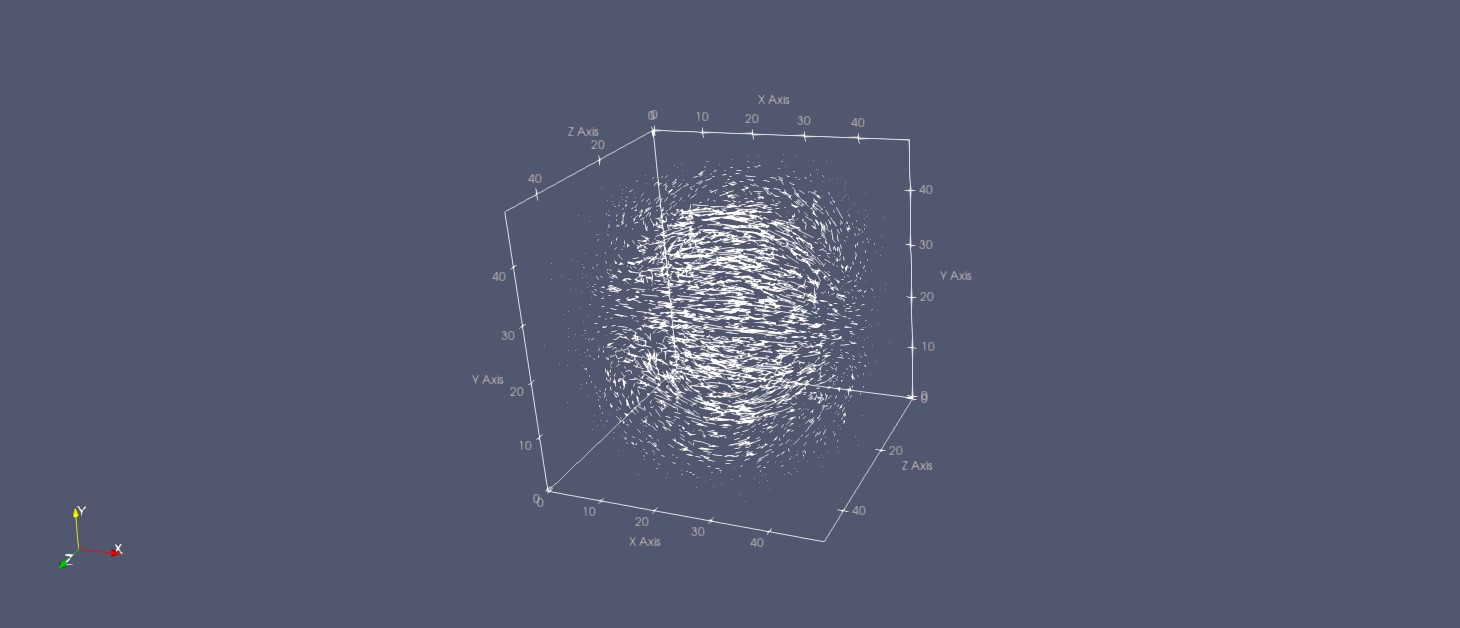
\includegraphics[width=.95\linewidth]{Figures/FDTD3DE1}
		\caption{t = 50}
	\end{subfigure}
	\begin{subfigure}{.49\textwidth}
		\centering
		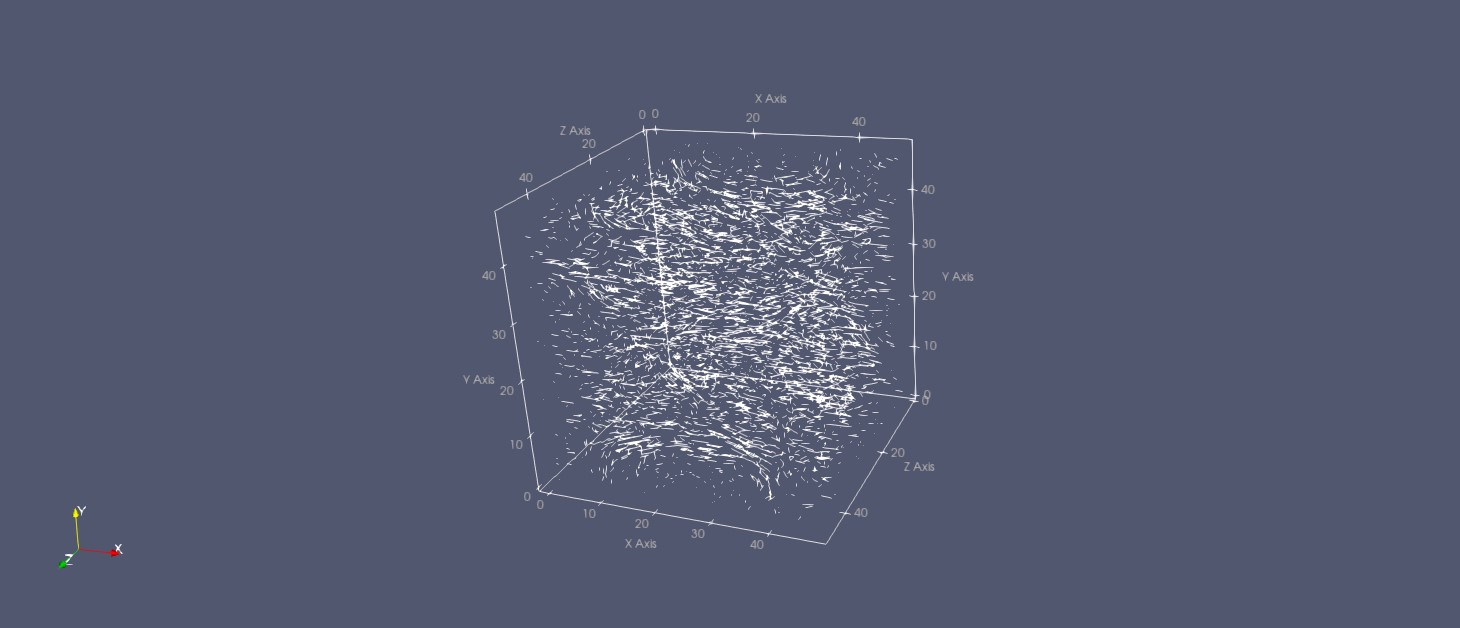
\includegraphics[width=.95\linewidth]{Figures/FDTD3DE2}
		\caption{t = 100}
	\end{subfigure}
	\begin{subfigure}{.49\textwidth}
		\centering
		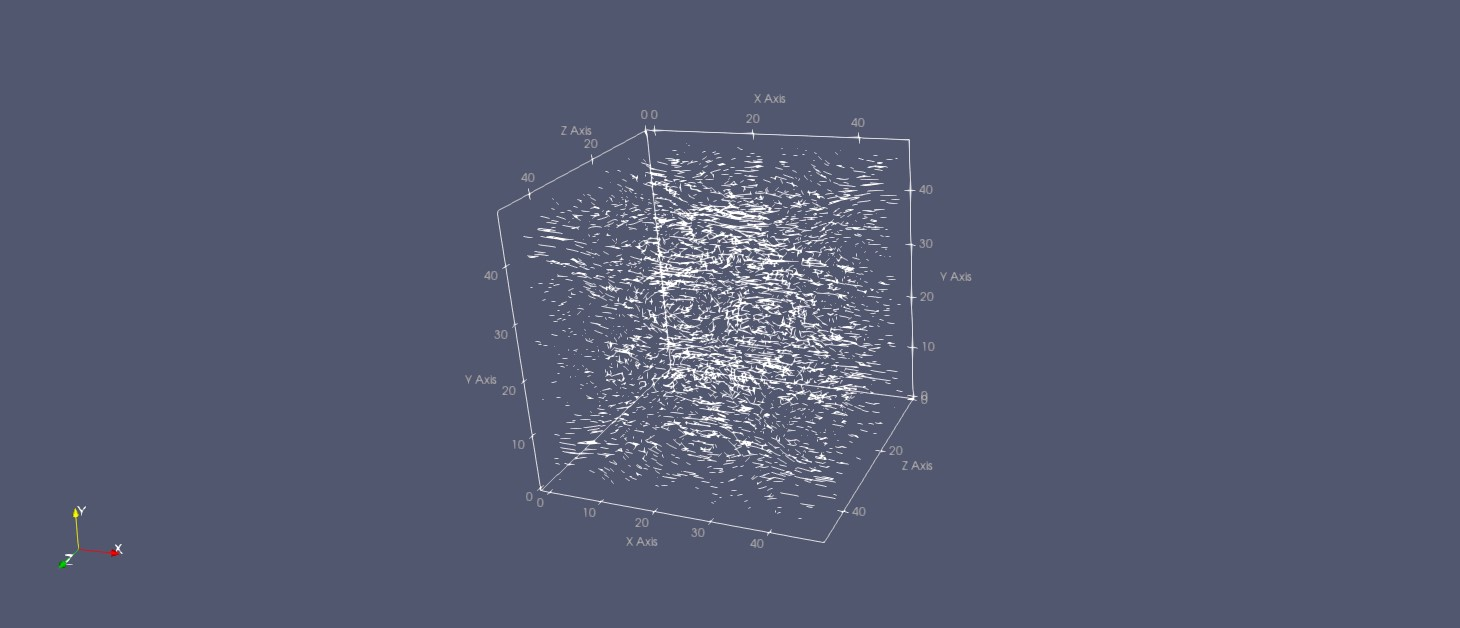
\includegraphics[width=.95\linewidth]{Figures/FDTD3DE3}
		\caption{t = 150}
	\end{subfigure}
	\begin{subfigure}{.49\textwidth}
		\centering
		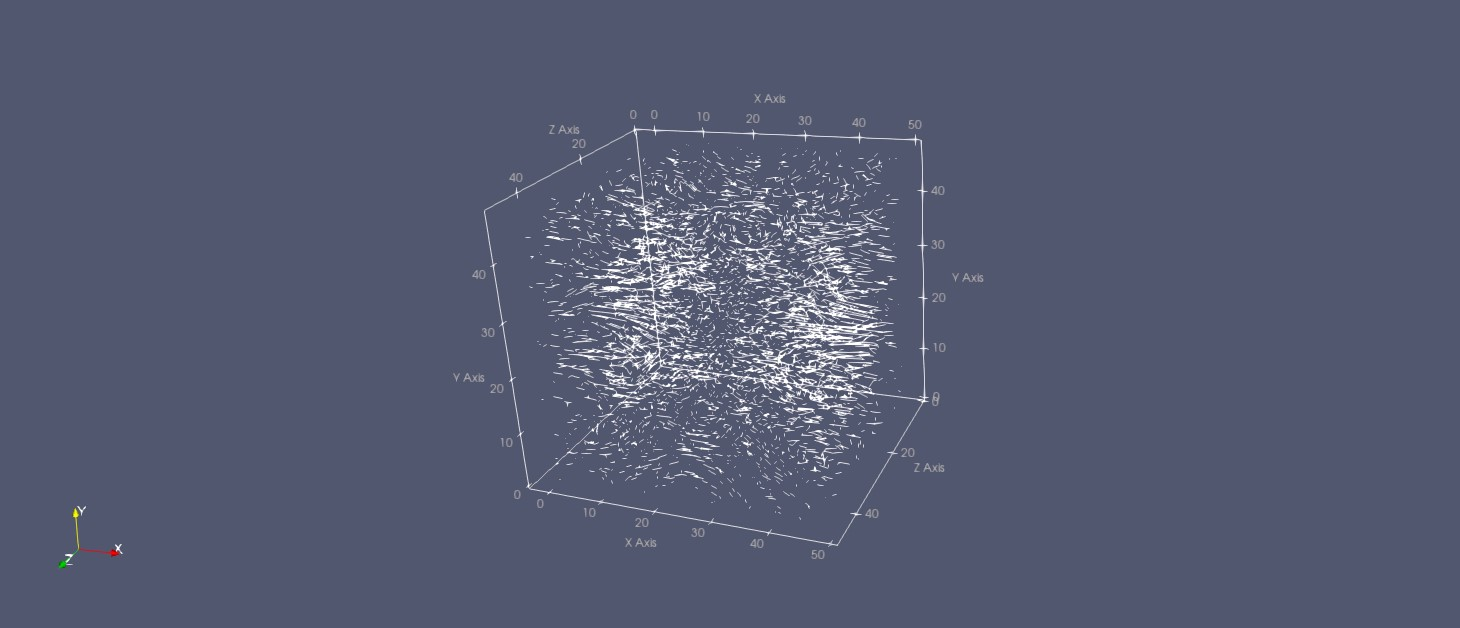
\includegraphics[width=.95\linewidth]{Figures/FDTD3DE4}
		\caption{t = 200}
	\end{subfigure}
	\decoRule
	\caption[3D Electric Field Simulation]{A simulation of the 3D electric field.}
	\label{fig:FDTD3DE}
\end{figure}

The same can be done for the magnetic data as well by following the same steps. It should be noted that this data will need to be scaled quite a bit more than its electric counterpart, as it would be quite hard to see otherwise due to using vacuum as the medium.

\begin{figure}[h!]
	\centering
	\begin{subfigure}{.49\textwidth}
		\centering
		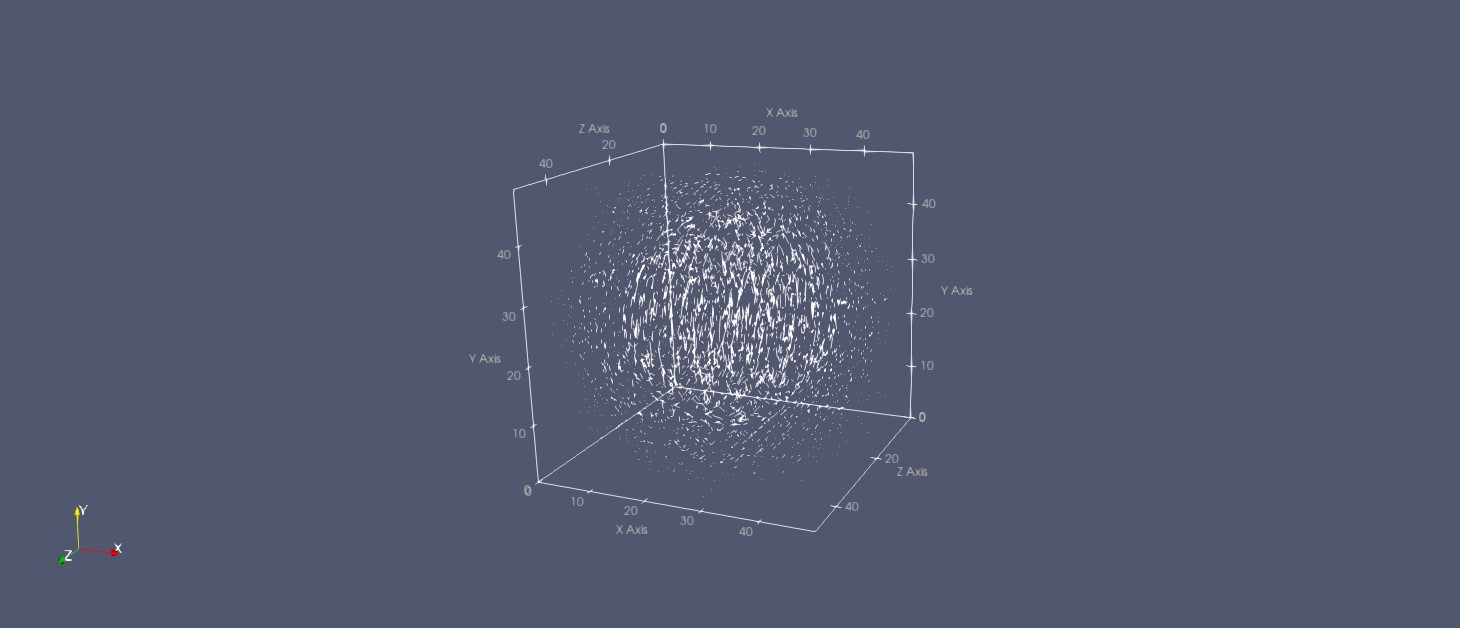
\includegraphics[width=.95\linewidth]{Figures/FDTD3DH1}
		\caption{t = 200}
	\end{subfigure}
	\begin{subfigure}{.49\textwidth}
		\centering
		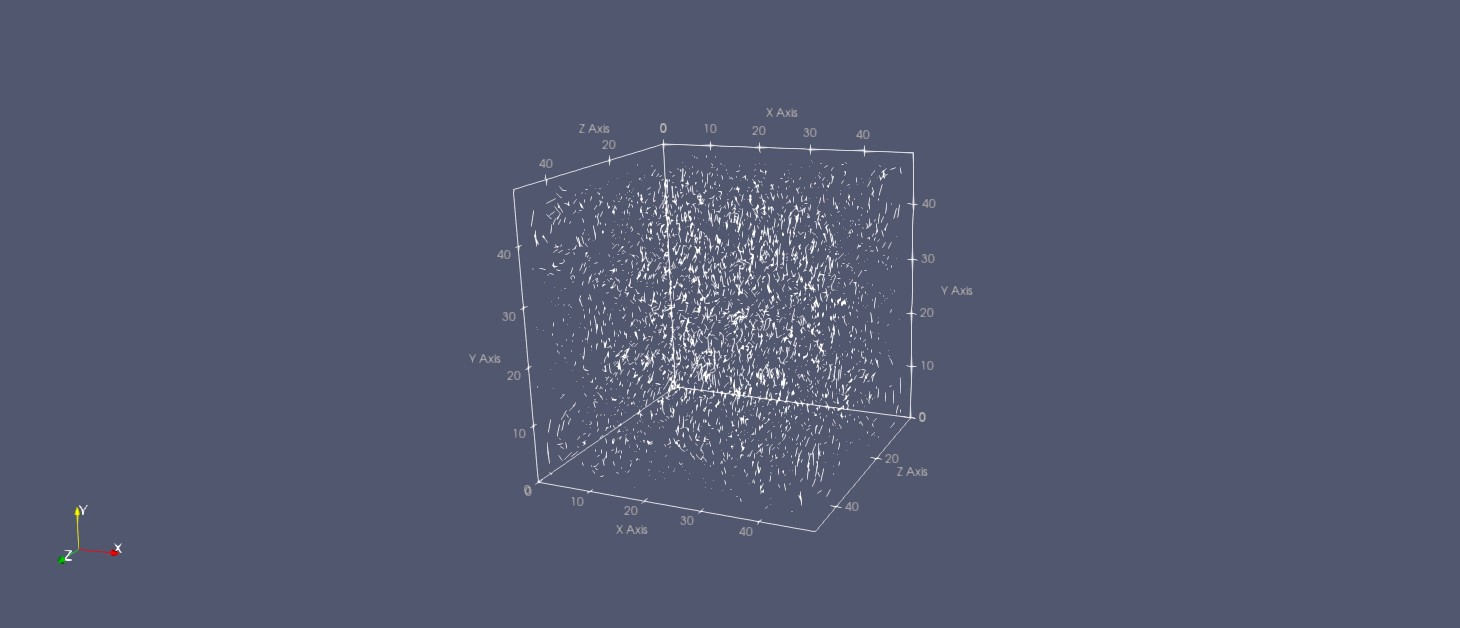
\includegraphics[width=.95\linewidth]{Figures/FDTD3DH2}
		\caption{t = 400}
	\end{subfigure}
	\begin{subfigure}{.49\textwidth}
		\centering
		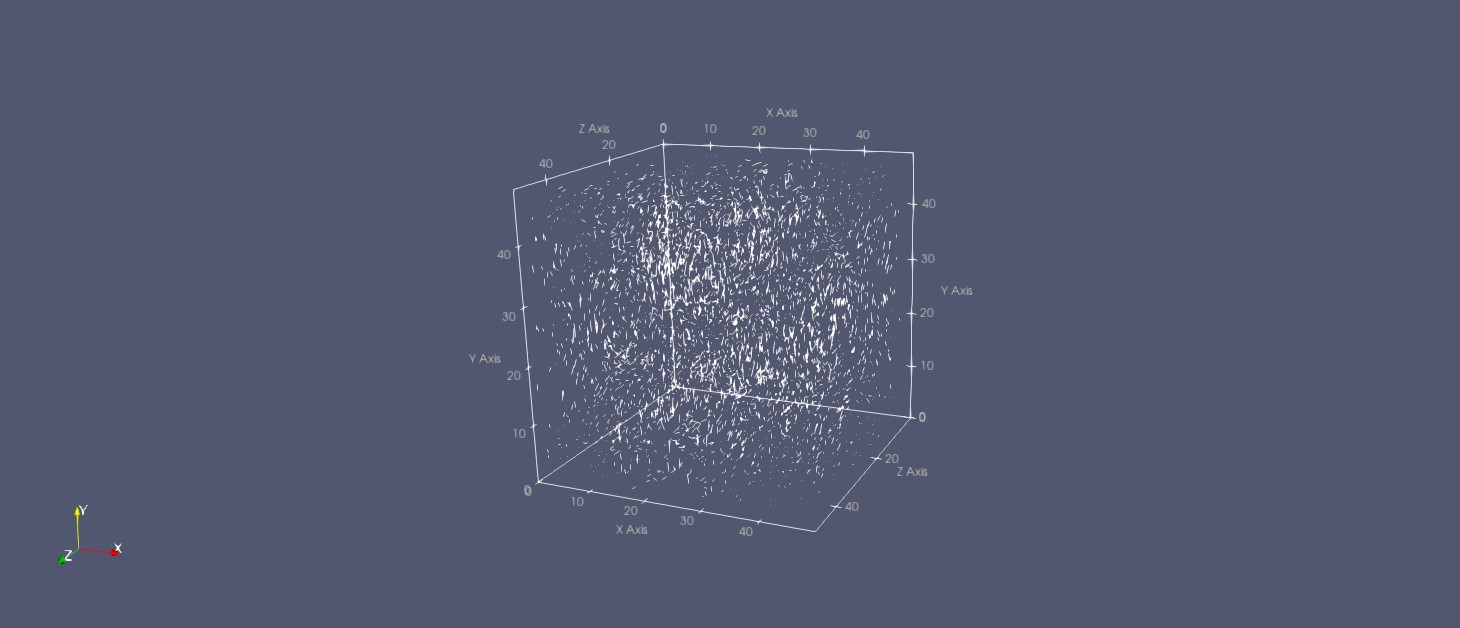
\includegraphics[width=.95\linewidth]{Figures/FDTD3DH3}
		\caption{t = 600}
	\end{subfigure}
	\begin{subfigure}{.49\textwidth}
		\centering
		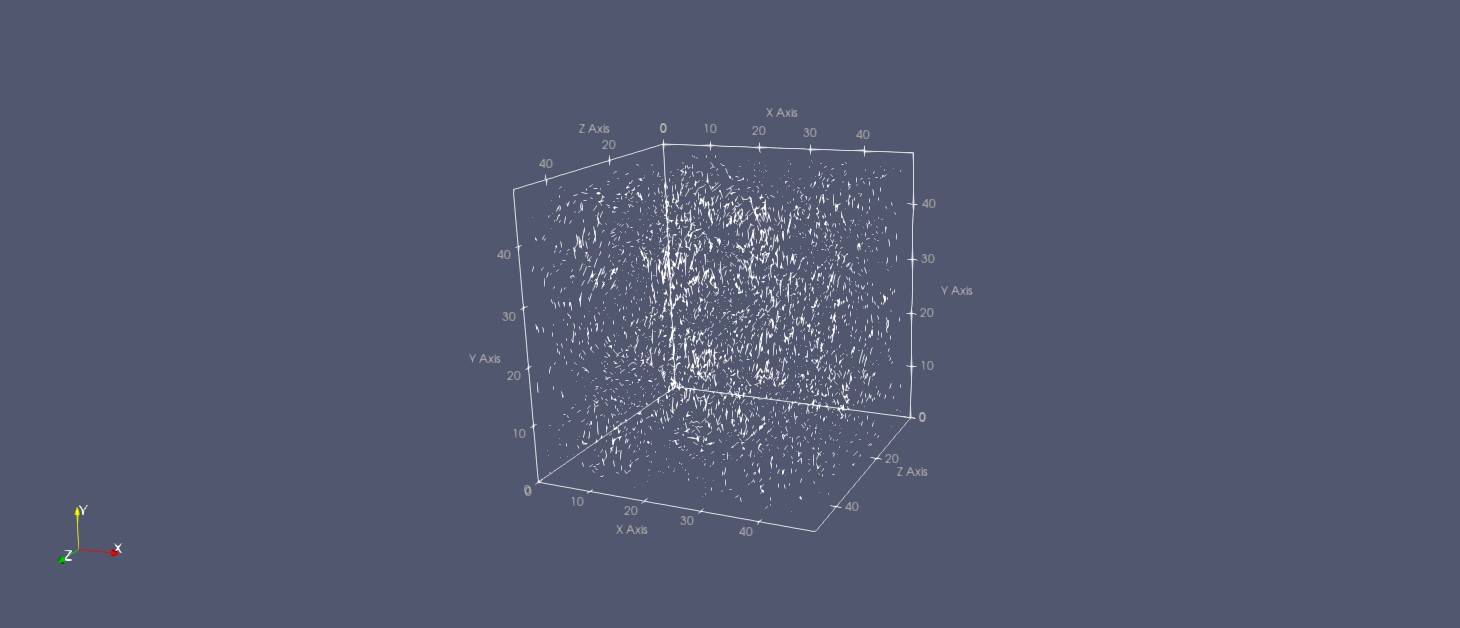
\includegraphics[width=.95\linewidth]{Figures/FDTD3DH4}
		\caption{t = 800}
	\end{subfigure}
	\decoRule
	\caption[3D Magnetic Field Simulation]{A simulation of the 3D magnetic field.}
	\label{fig:FDTD3DH}
\end{figure}

With that, the simulation for a three-dimensional scenario, and also this project as a whole, is complete. 